\documentclass[tikz,border=5pt]{standalone}
\usetikzlibrary{bending,angles,quotes}
\usepackage{fourier}
\begin{document}
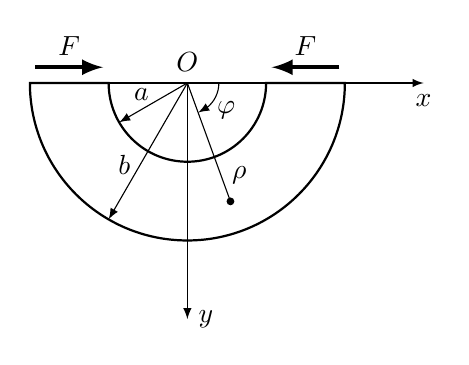
\begin{tikzpicture}[>=latex,label distance=-3pt]
\draw[->] (-2,0) -- (3,0) node[label={below:$x$}] (x) {};
\draw[->] (0,0) -- (0,-3) node[label={right:$y$}] {};
\draw[thick](-2,0) -- (-1,0) arc(180:360:1) -- (2,0) arc(360:180:2) -- cycle;
\draw(0,0) node[label={above:$O$}] (O) {} -- (-70:1.6) node[pos=.9,label={[label distance=-7pt]above right:$\rho$}] (rho) {} node[inner sep=1pt,fill,circle] {};
\draw[ultra thick,->,shorten <=2pt,shorten >=2pt] (-2,.2) -- node[above] {$F$} ++(1,0);
\draw[ultra thick,->,shorten <=2pt,shorten >=2pt] (2,.2) -- node[above] {$F$} ++(-1,0); 
\pic["$\varphi$",draw,<-,angle radius=.4cm,angle eccentricity=1.5] {angle=rho--O--x};
\draw[->] (0,0) -- node[left=3pt,pos=.3] {$a$} (-150:1);
\draw[->] (0,0) -- node[left,pos=.6] {$b$} (-120:2);
\end{tikzpicture}
\end{document}